%\subsection{域适配问题 (domain adaptation)}
\begin{frame}
    \frametitle{迁移学习:域适配问题}
    \begin{itemize}
        \item 域适配问题
            \begin{itemize}
                \item domain adaptation, cross-domain learning
                \item 问题定义:有标签的源域和无标签的目标域共享相同的特征和类别,但是特征分布不同,如何利用源域标定目标域.
                $\mathcal{D}_S \neq \mathcal{D}_T: P_S(X) \neq P_T(X)$
            \end{itemize}
    \end{itemize}
    \begin{figure}
        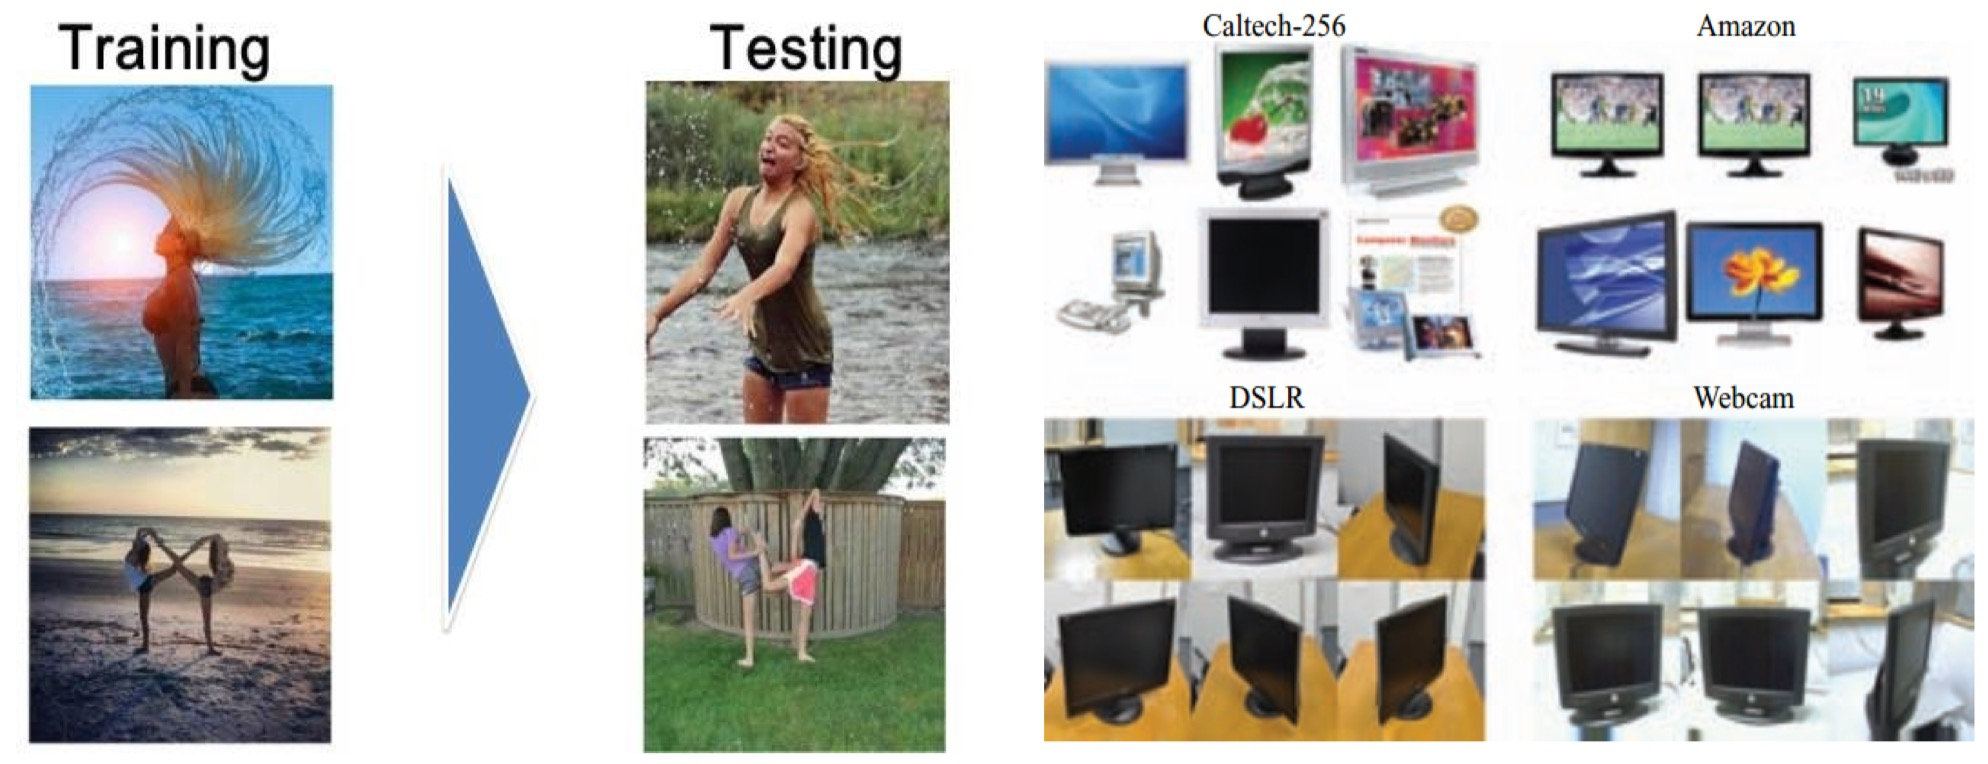
\includegraphics[width=0.9\textwidth]{da.jpg}
    \end{figure}
\end{frame}

\begin{frame}
    \frametitle{迁移学习:域适配问题}
    \begin{itemize}
        \item 域适配问题
            \begin{itemize}
                \item 基于特征的迁移方法:
                    \begin{itemize}
                        \item Transfer component analysis [Pan, TKDE-11]
                        \item Geodesic flow kernel [Duan, CVPR-12]
                        \item Transfer kernel learning [Long, TKDE-15]
                        \item TransEMDT [Zhao, IJCAI-11]
                    \end{itemize}
                \item 基于实例的迁移方法:
                    \begin{itemize}
                        \item Kernel mean matching [Huang, NIPS-06]
                        \item Covariate Shift Adaptation [Sugiyama, JMLR-07]
                    \end{itemize}
                \item 基于模型的迁移方法:
                    \begin{itemize}
                        \item Adaptive SVM (ASVM) [Yang et al, ACM Multimedia-07]
                        \item Multiple Convex Combination (MCC) [Schweikert, NIPS-09]
                        \item Domain Adaptation Machine (DAM) [Duan, TNNLS-12]
                    \end{itemize}
            \end{itemize}
    \end{itemize}
\end{frame}

\begin{frame}
    \frametitle{迁移学习:域适配问题}
    \begin{itemize}
        \item 迁移成分分析 (TCA, transfer component analysis) \footfullcite{ijcai2009-200}
            \begin{itemize}
                \item 将源域和目标域变换到相同空间,最小化它们的距离
            \end{itemize}
    \end{itemize}
    \begin{figure}
        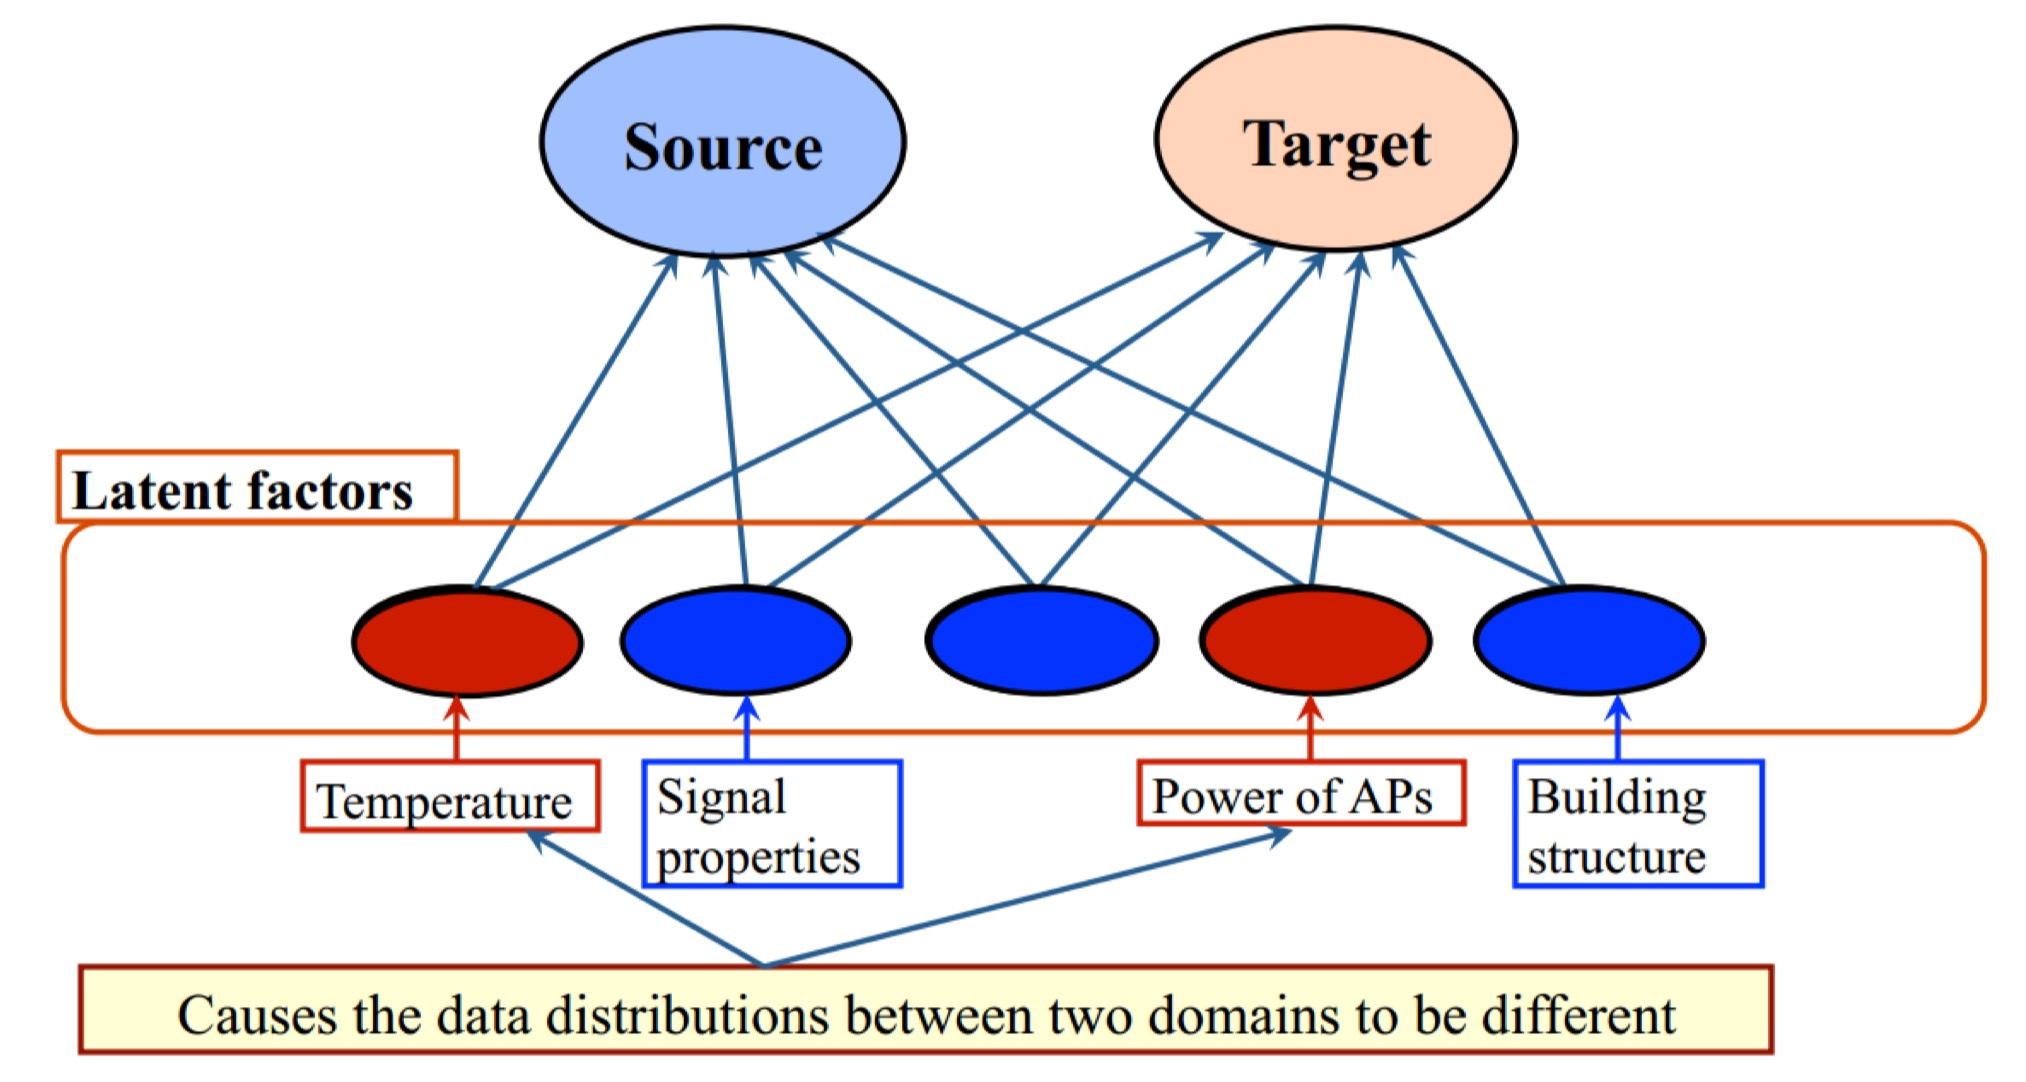
\includegraphics[width=0.9\textwidth]{tca.jpg}
    \end{figure}
\end{frame}

\begin{frame}
    \frametitle{迁移学习:域适配问题}
    \begin{itemize}
        \item 迁移成分分析 (TCA, transfer component analysis)
            \begin{itemize}
                \item 优化目标 (s.t. constraints on $\varphi(X_S)$, $\varphi(X_T)$)
                $$\max_{\varphi}\  \text{Dist}(\varphi(X_S),\varphi(X_T)) + \lambda \Omega(\varphi)$$
                \item Maximum mean discrepancy (MMD)
                $$\text{Dist}[P(X_S),P(X_T)] \triangleq\Vert \frac{1}{n_S}\sum\limits_{i=1}^{n_S}\phi(x_{S_i})-\frac{1}{n_T}\sum\limits_{j=1}^{n_T}\phi(x_{T_j})\Vert_{\mathcal{H}}$$
            \end{itemize}
    \end{itemize}
    \begin{figure}
        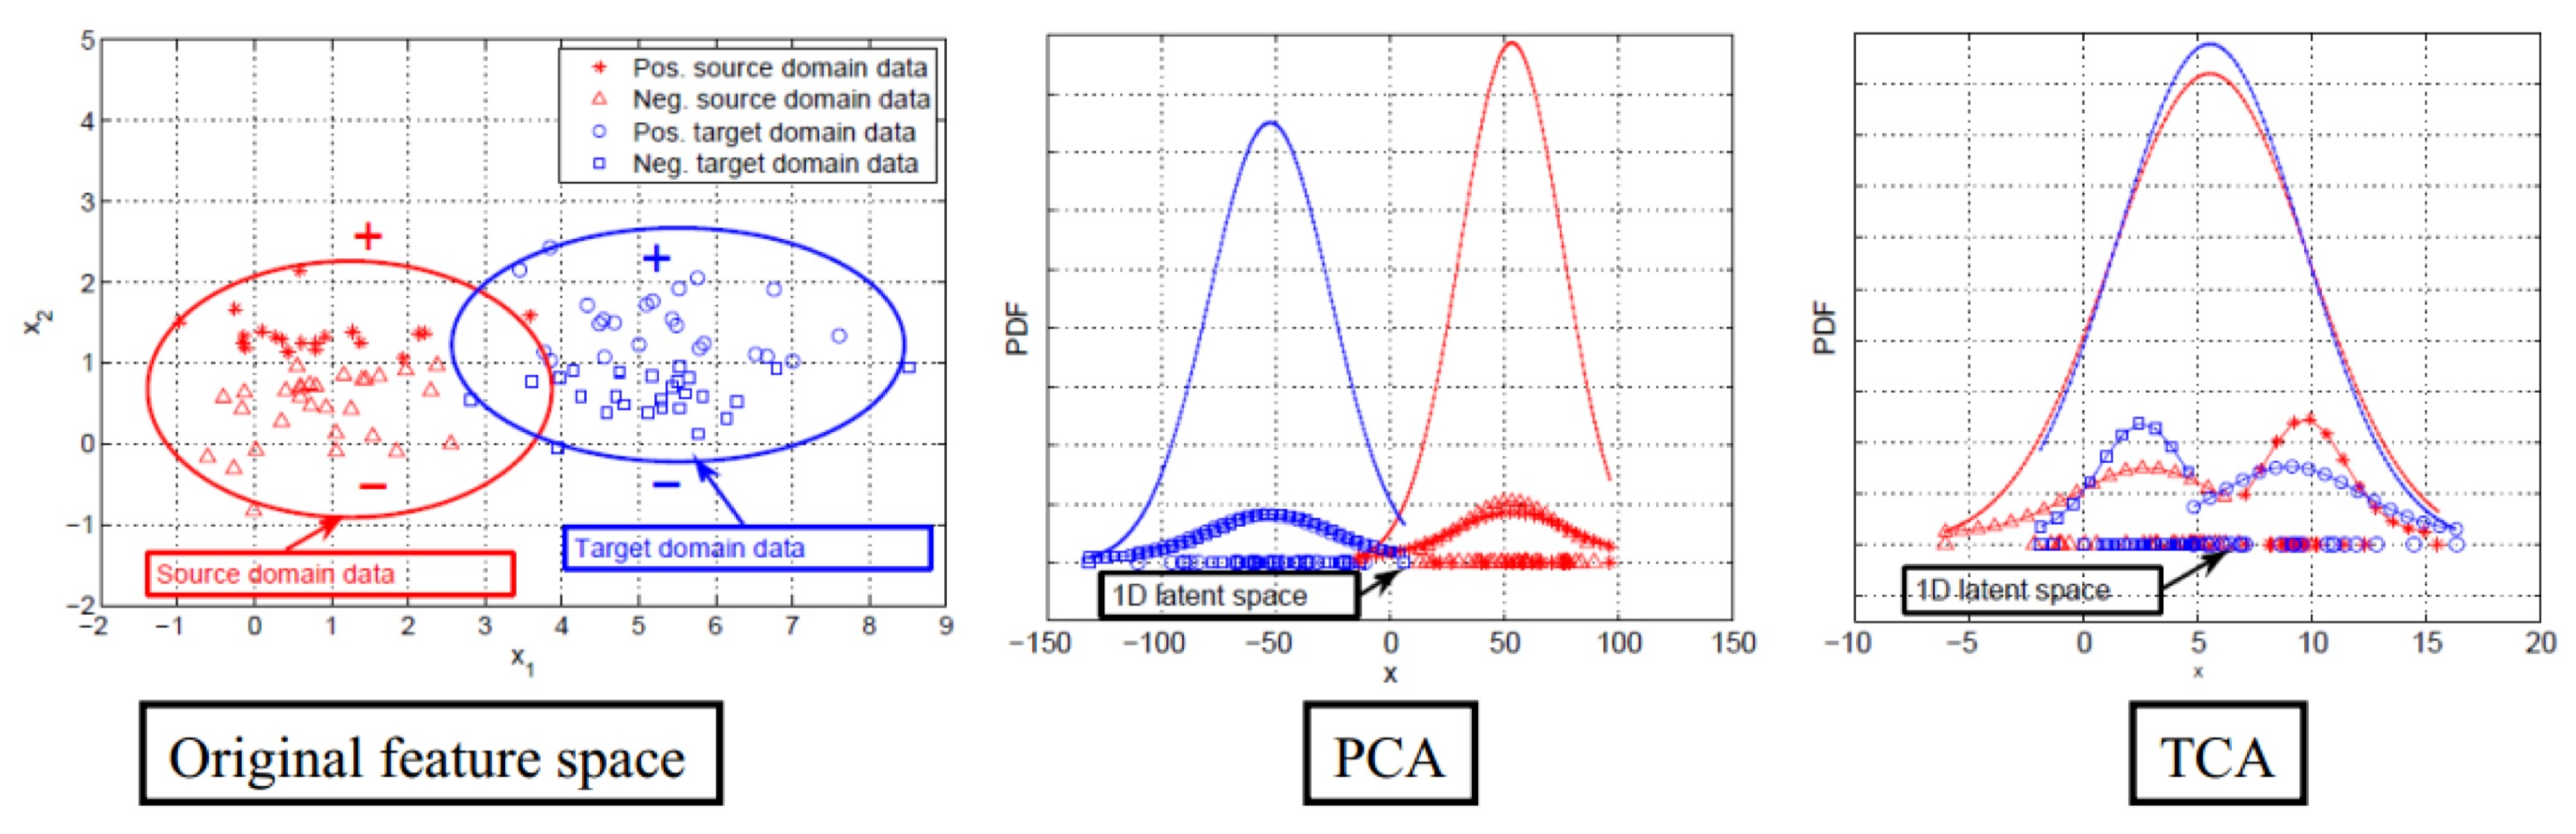
\includegraphics[width=0.8\textwidth]{tca2.jpg}
    \end{figure}
\end{frame}

\begin{frame}
    \frametitle{迁移学习:域适配问题}
    \begin{itemize}
        \item GFK (geodesic flow kernel) \footfullcite{gong2012geodesic}
            \begin{itemize}
                \item 利用流形学习,将数据映射到高维空间中,然后测量其距离 ,使得源域和目标域差异最大
                \item 优化目标
                    $$\Phi(t)=P_S U_1\Gamma(t) - R_S U_2\Sigma(t)$$
                    $$P_S^T P_{\mathcal{T}} = U_1 \Gamma V^T, R_S^T P_{\mathcal{T}} = -U_2 \Sigma V^T$$
                \item 流形正则项
                $\mathcal{R(S,T)} = \frac{1}{d^*} \sum_i^{d^*} \theta_i[\text{KL}(\mathcal{S}_i\parallel \mathcal{T}_i) + \text{KL}(\mathcal{T}_i\parallel \mathcal{S}_i)]
                $
            \end{itemize}
    \end{itemize}
    \begin{figure}
        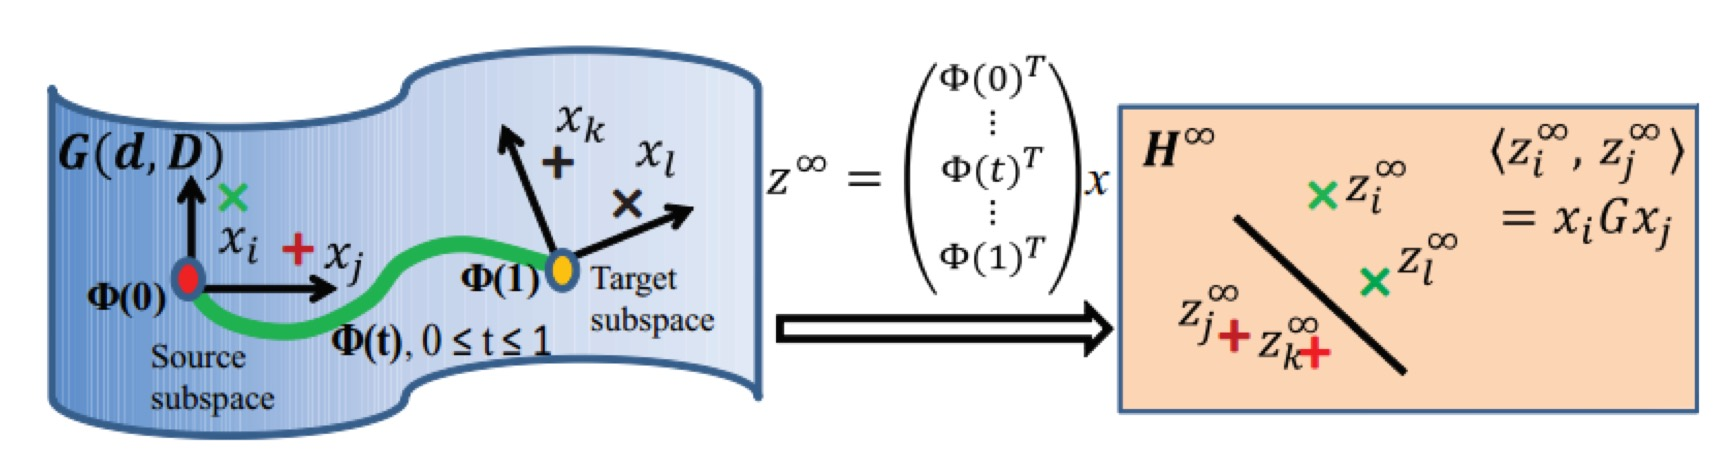
\includegraphics[width=0.7\textwidth]{gfk.jpg}
    \end{figure}
\end{frame}

\begin{frame}
    \frametitle{迁移学习:域适配问题}
    \begin{itemize}
        \item Transfer Kernel Learning (TKL) \footfullcite{long2015domain}
            \begin{itemize}
                \item 在再生核希尔伯特空间中学习一个领域不变核矩阵,从而实现源域和目标域的适配
                \item 优化目标
                $$\min_{\Lambda} \lVert \bar{\mathbf{K}}_{\mathcal Z} - \mathbf{K}_{\mathcal Z} \rVert^2_F = \lVert \bar{\Phi}_{\mathcal{Z}} \Lambda
\bar{\Phi}_{\mathcal{Z}}^{\text{T}}- \mathbf{K}_{\mathcal Z} \rVert ^2_F $$
                $$\lambda_i \geq \zeta\lambda_{i+1}, i=1,...,n-1$$
                $$\lambda_i \geq 0, i=1,...,n$$
            \end{itemize}
    \end{itemize}
    \begin{figure}
        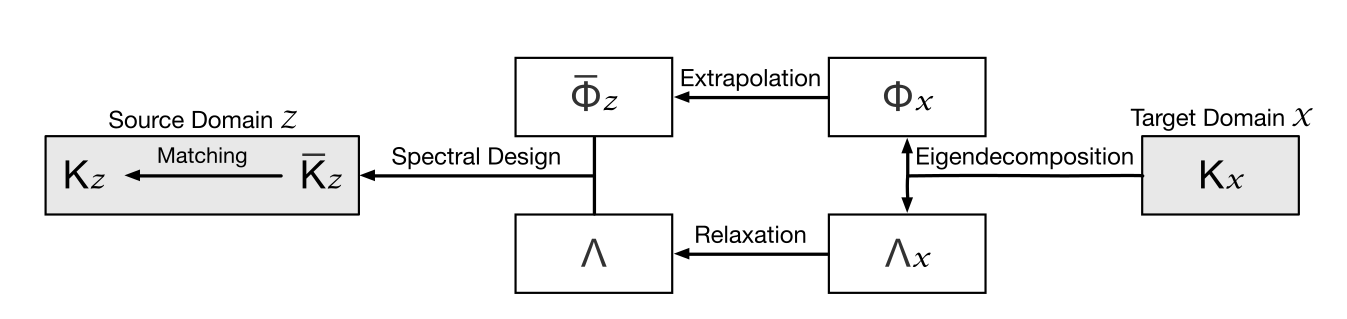
\includegraphics[width=0.9\textwidth]{tkl.png}
    \end{figure}
\end{frame}

\begin{frame}
    \frametitle{迁移学习:域适配问题}
    \begin{itemize}
        \item 嵌入决策树算法 (TransEMDT) \footfullcite{zhao2011cross}
            \begin{itemize}
                \item 首先通过聚类得到初始的目标域决策树模型,然后迭代更新决策树的参数直到收敛为止
            \end{itemize}
    \end{itemize}
    \begin{figure}
        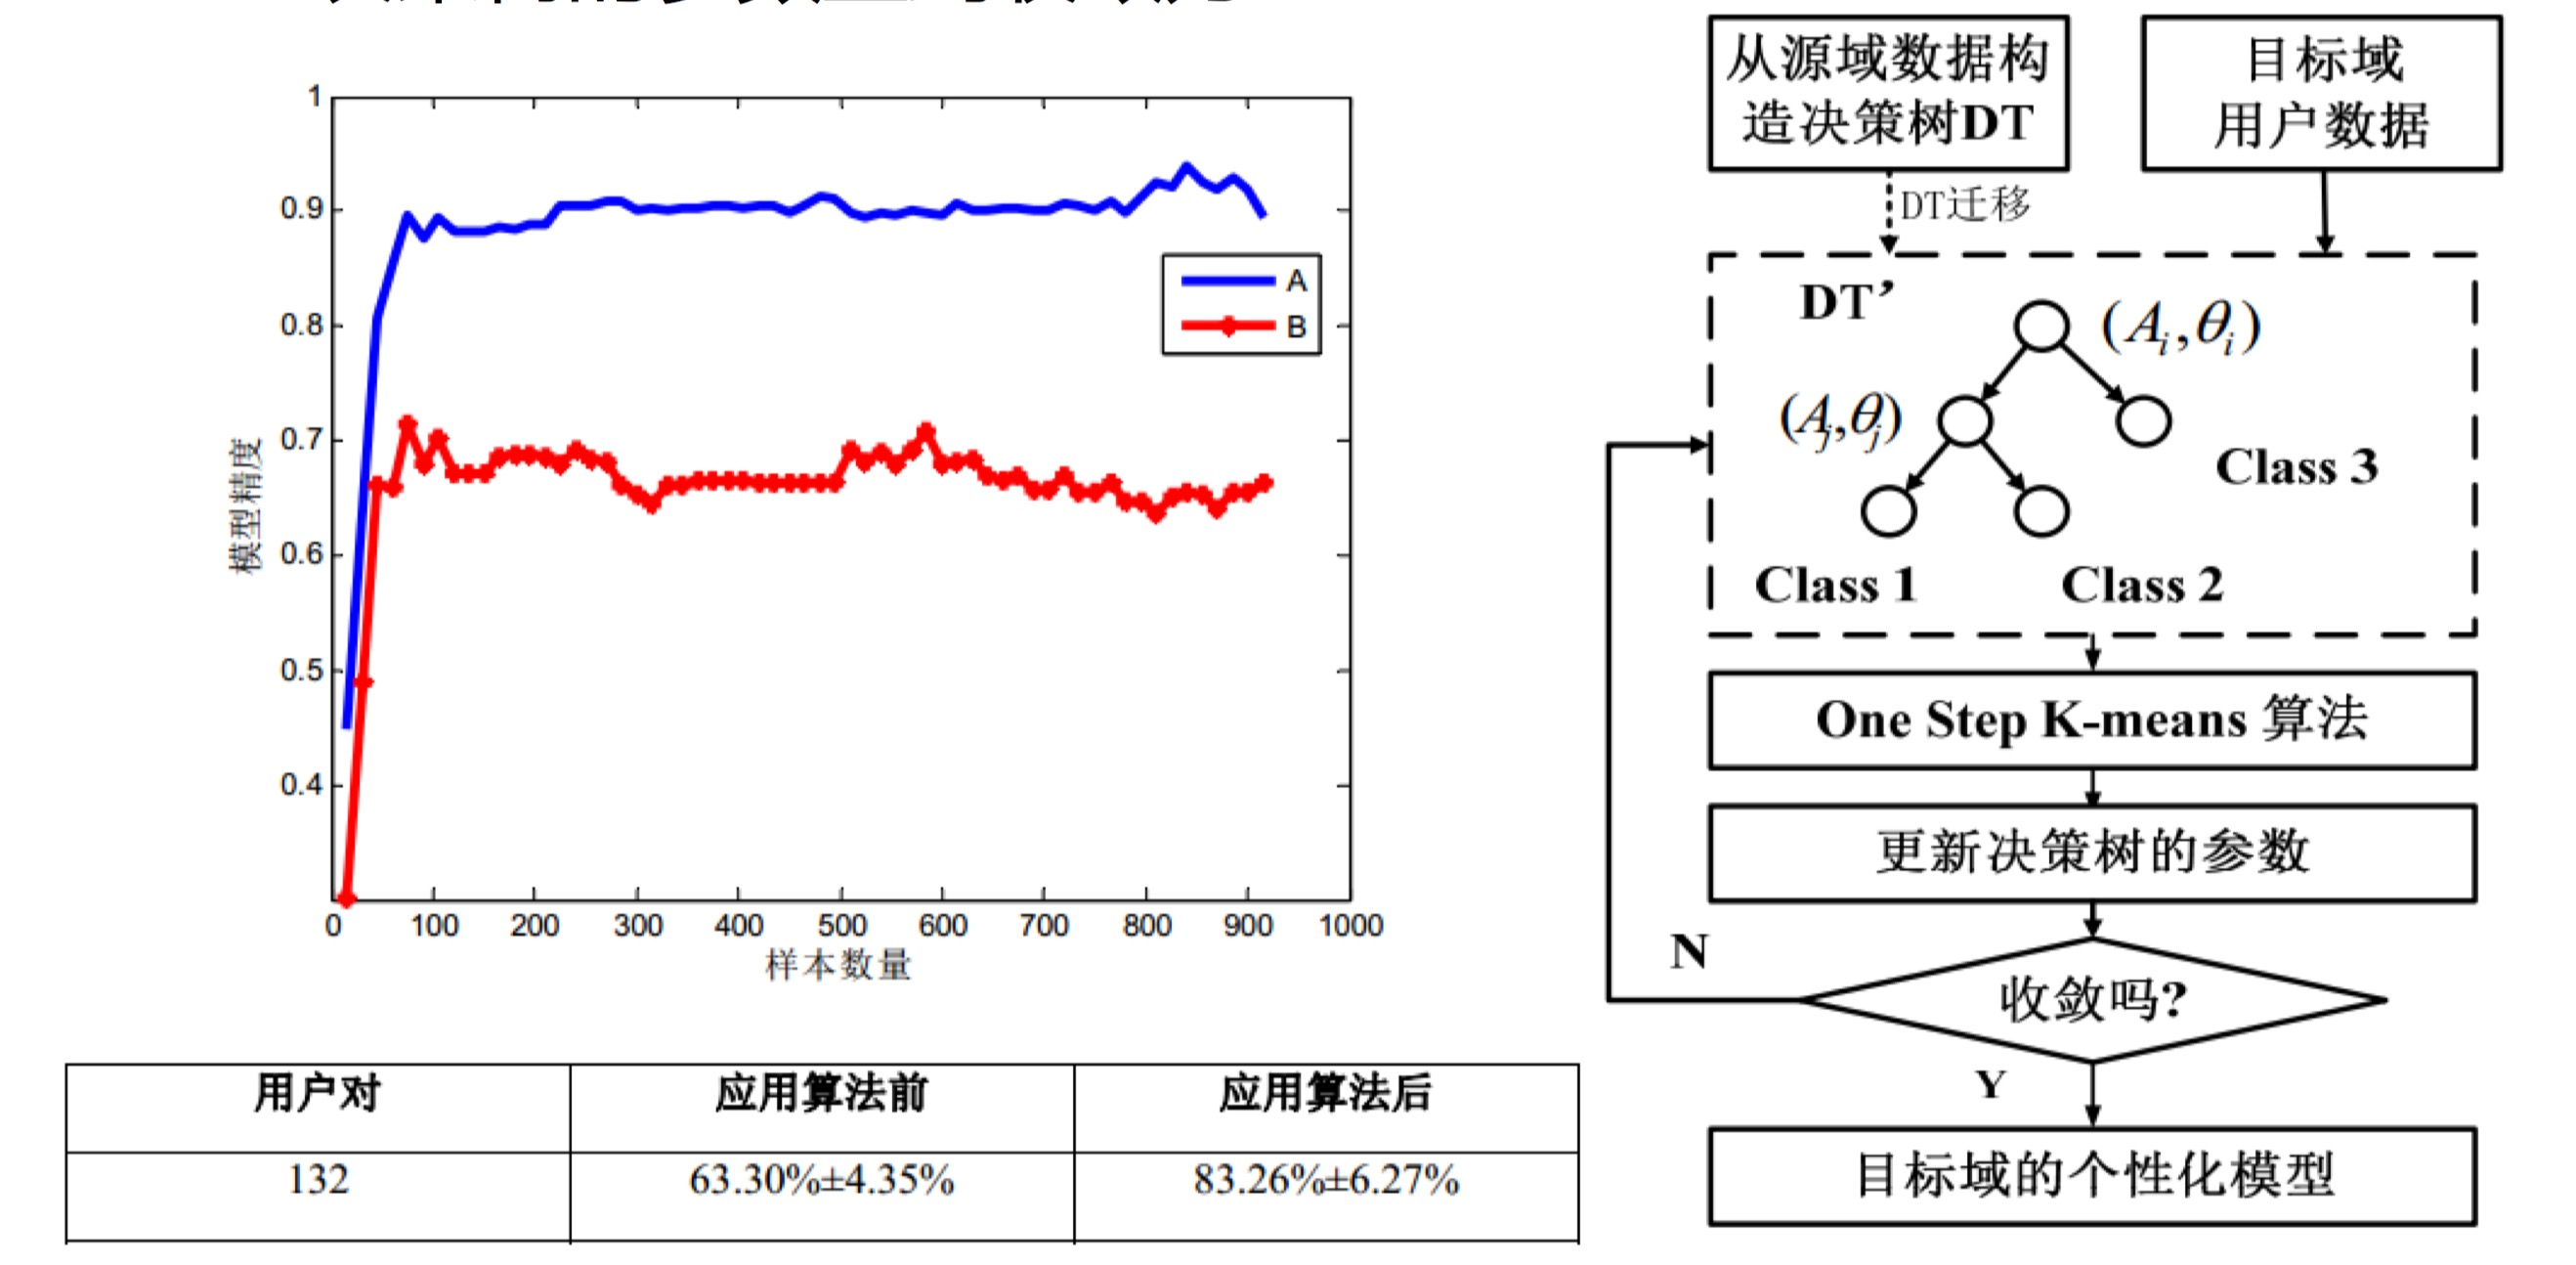
\includegraphics[width=0.9\textwidth]{tremdt.jpg}
    \end{figure}
\end{frame}

\begin{frame}
    \frametitle{迁移学习:域适配问题}
    \begin{itemize}
        \item Kernel mean matching \footfullcite{huang2007correcting}
            \begin{itemize}
                \item 在再生希尔伯特空间中计算源域和目标域的协方差分布差异 ,然后用二次规划求解样本权重
                \item 优化目标
            \end{itemize}
    \end{itemize}
    \begin{figure}
        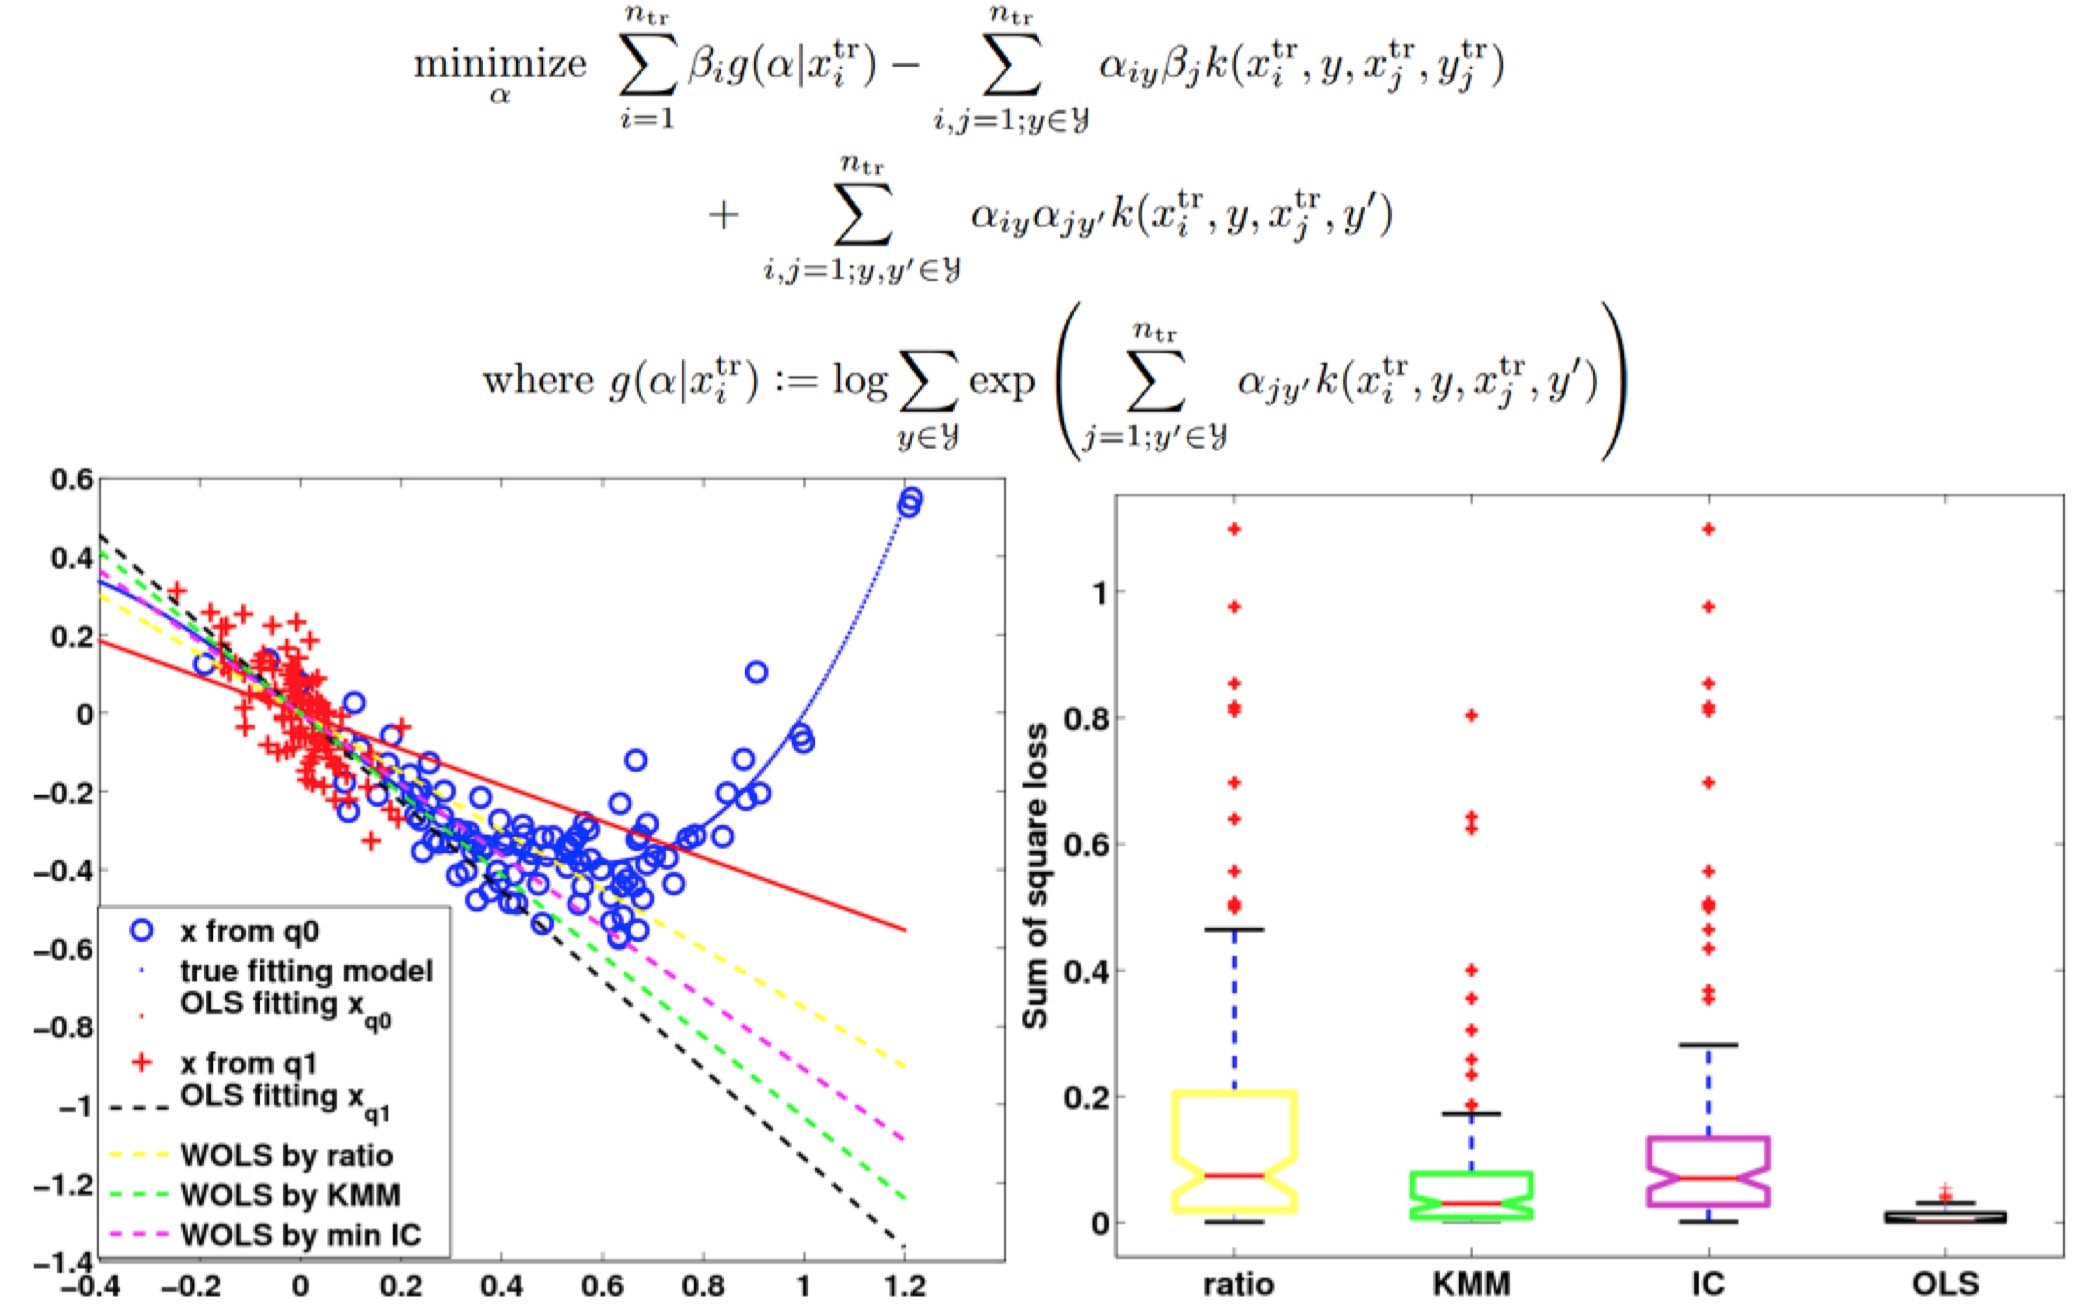
\includegraphics[width=0.6\textwidth]{kmm.jpg}
    \end{figure}
\end{frame}

\begin{frame}
    \frametitle{迁移学习:域适配问题}
    \begin{itemize}
        \item Covariate Shift Adaptation \footfullcite{wu2013learning}
            \begin{itemize}
                \item 采用自然估计法估计源域和目标域的密度比例,然后进行实 例权重的分配,最后迁移
                \item 优化目标
            \end{itemize}
    \end{itemize}
    \begin{figure}
        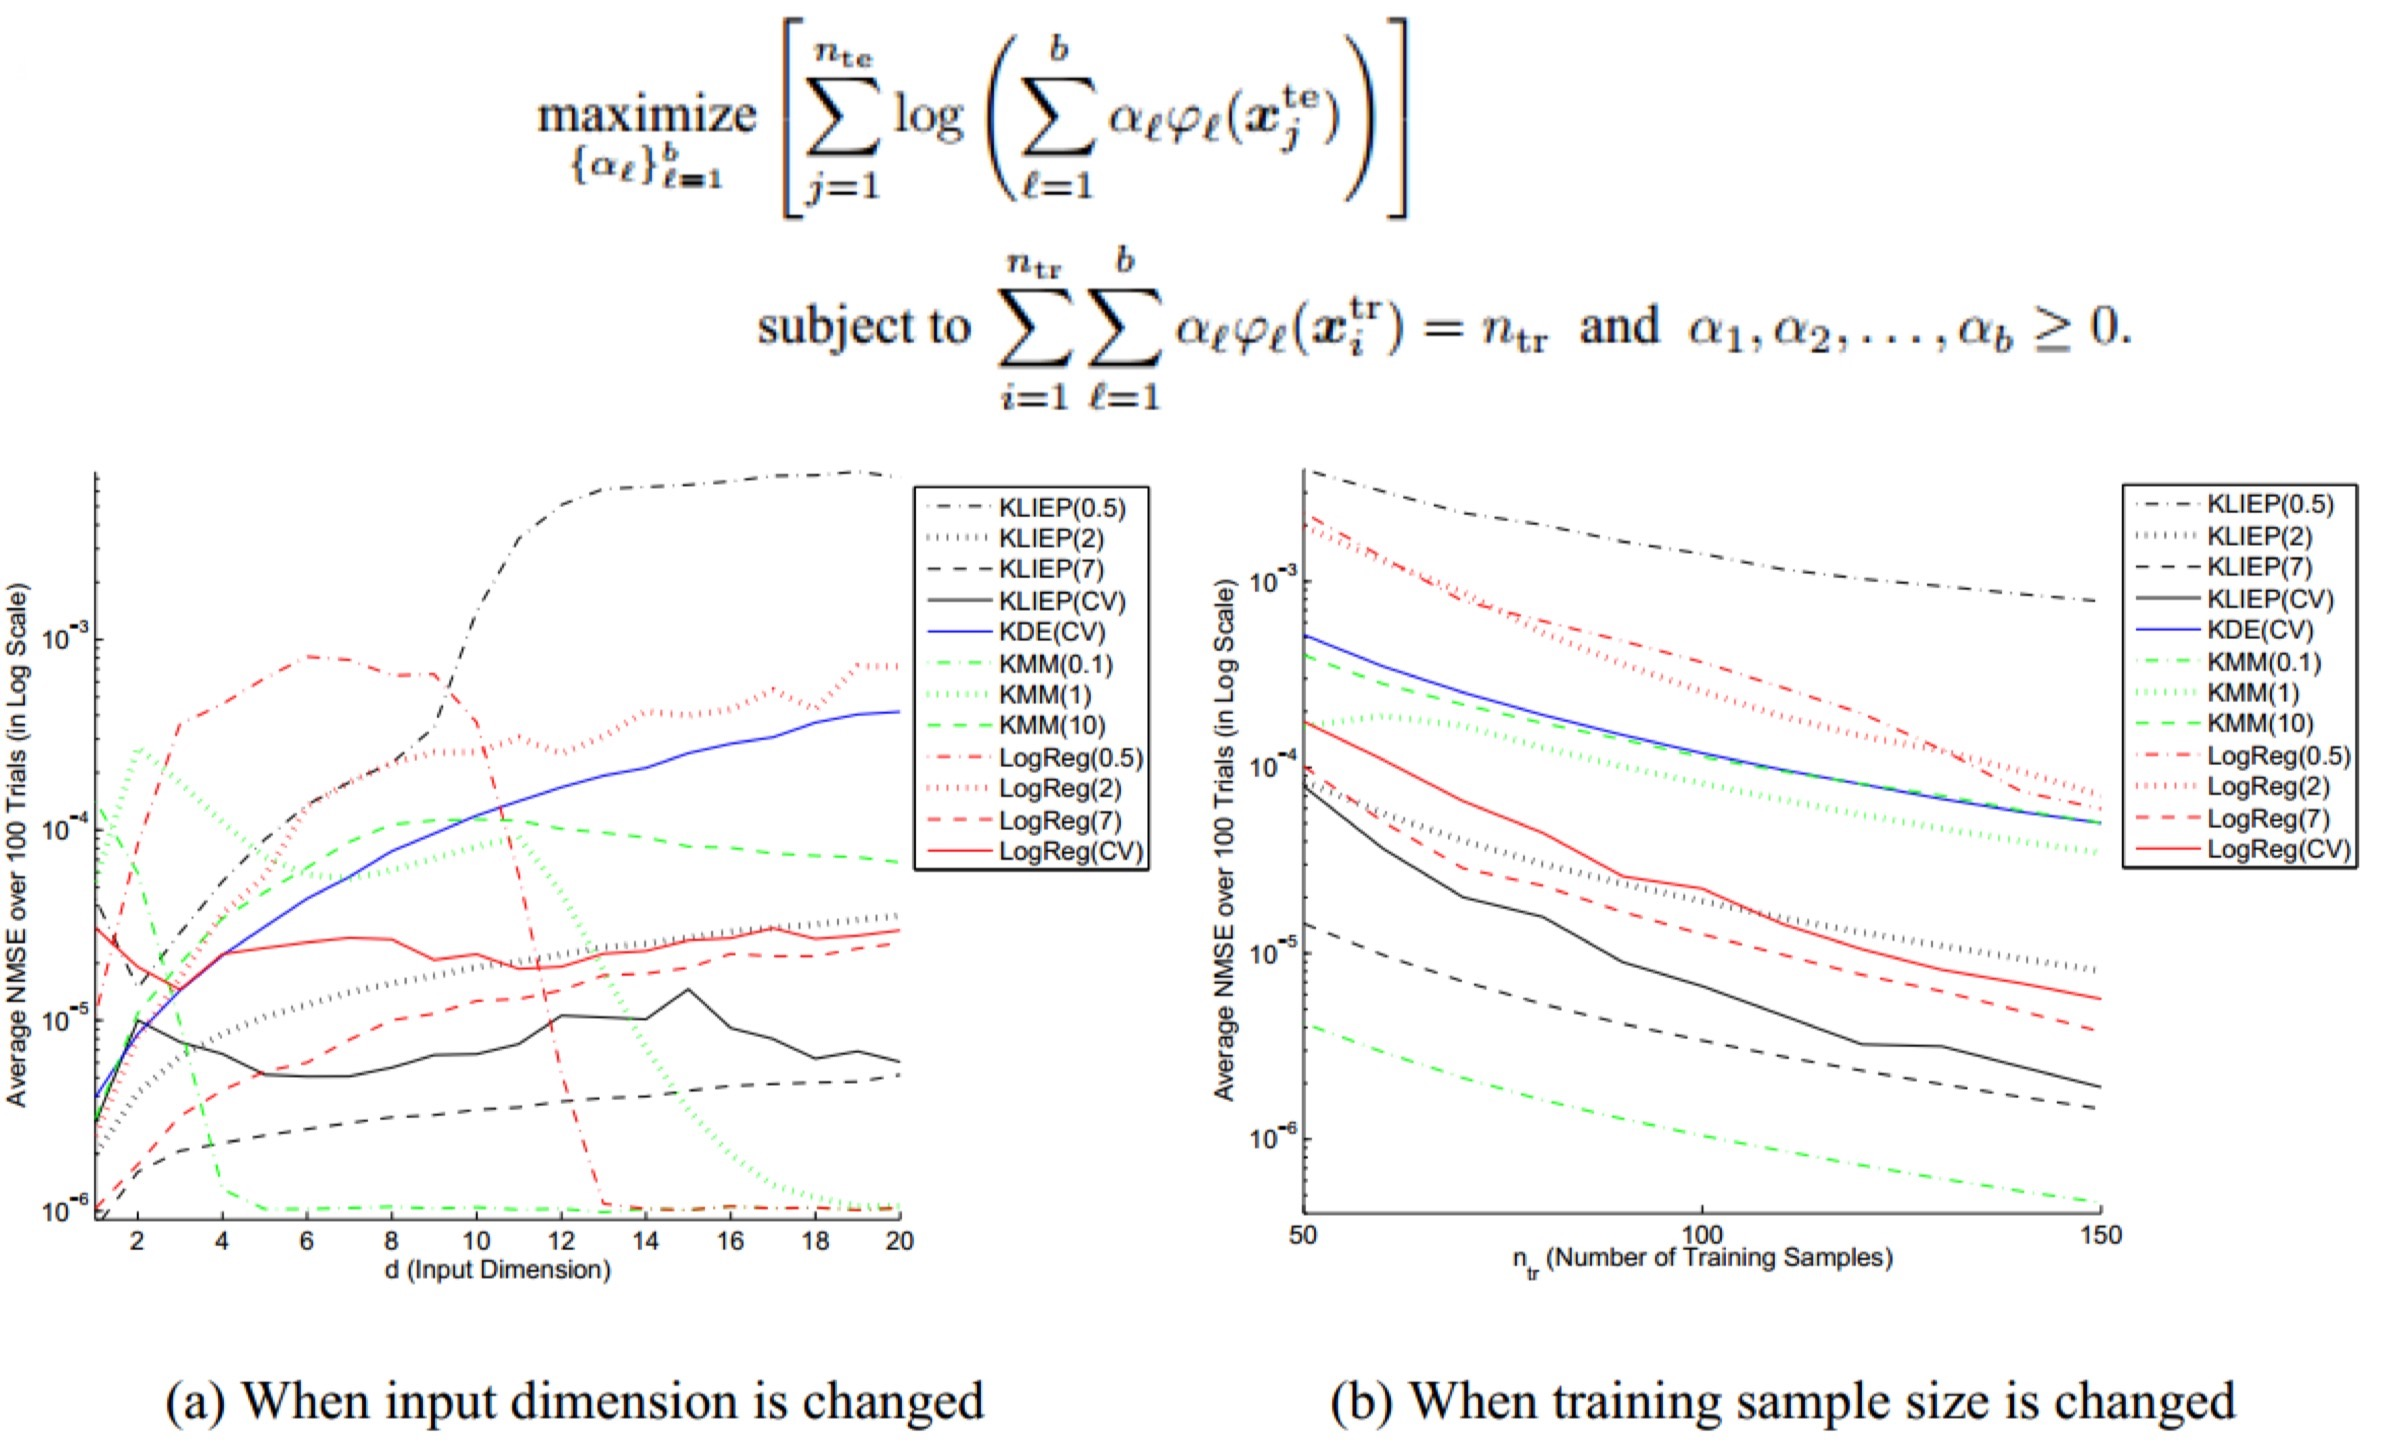
\includegraphics[width=0.7\textwidth]{csa.jpg}
    \end{figure}
\end{frame}

\begin{frame}
    \frametitle{迁移学习:域适配问题}
    \begin{itemize}
        \item 总结
        \begin{itemize}
            \item 通常假设源域和目标域的数据有着相同的条件分布,或者在高维空间里,有着相同的条件分布
            \item 这个假设是有一定局限性的,无法衡量源域和目标域之间相 似性,可能发生负迁移
        \end{itemize}
    \end{itemize}
\end{frame}